
\section{Motivating Scenario}
\label{sec:motivation}

Consider the complex multi-tier service-oriented system shown in Figure \ref{fig:motivation} that contains several interacting services (web servers, application servers, search and indexing, database, etc.). 
The system is maintained by operators who can observe the health of the system using lightweight monitoring that is attached to the deployed system.
\xxx{Still need some statement here that it's reasonable to assume that they are already running each tier in its own container... This is an important one...}
%In the interest of application performance, production system monitoring is usually limited to system resource usage, application usage statistics, transaction logs, and error logs.
At some point, an unusual memory usage is observed in the glassfish application server, and some error logs are generated in the Nginx web server. 
Administrators can then surmise that there is a potential memory leak/allocation problem in the app-server or a problem in the web server.
However, with a limited amount of monitoring information, they can only go so far.


Typically, trouble tickets are generated for such problems, and they are debugged offline.
However using \parikshan, administrators can generate replicas of the Nginx and Glassfish containers as \textbf{\textit{Nginx-debug}} and \textbf{\textit{glassfish-debug}}.
\parikshan's network duplication mechanism ensures that the debug replicas receive the same inputs as the production containers and that the production containers continue to provide service without interruption.
This separation of the production and debug environment allows the operator to use dynamic instrumentation tools to perform deeper diagnosis without fear of additional disruptions due to debugging.
Since the replica is cloned from the original potentially ``buggy'' \productioncontainer, it will also exhibit the same memory leaks/or logical errors.
Additionally, \parikshan can focus on the ``buggy'' parts of the system, without needing to replicate the entire system in a test-cluster.
This process will greatly reduce the time to bug resolution, and allow real-time bug diagnosis capability.

The replica can be created at any time: either from the start of execution, or at any point during execution that an operator deems necessary, allowing for post-facto analysis of the error, by observing execution traces of incoming requests (in the case of performance bugs and memory leaks, these will be persistent in the running system).
Within the debug replica, the developer is free to employ any dynamic analysis tools to study the buggy execution, as long as the only side-effect those tools is on execution speed.
%\xxx{need to describe assumptions: debug is identical except for external timing/slowdowns (need to clarify what kind of debugging activities are permitted). assume that it's OK to use a VM as the container, and that it is 'free' to dos so}

\begin{figure*}[ht!]
	\begin{center}
		%    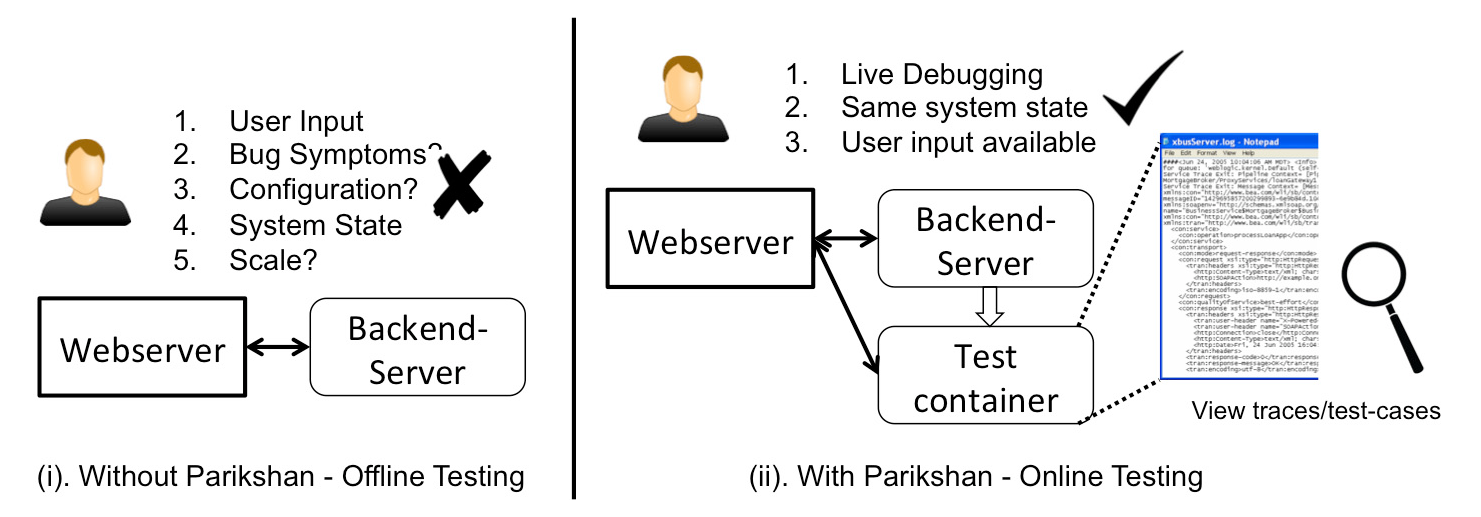
\includegraphics[width=0.7\textwidth]{figs/motivation.eps}
		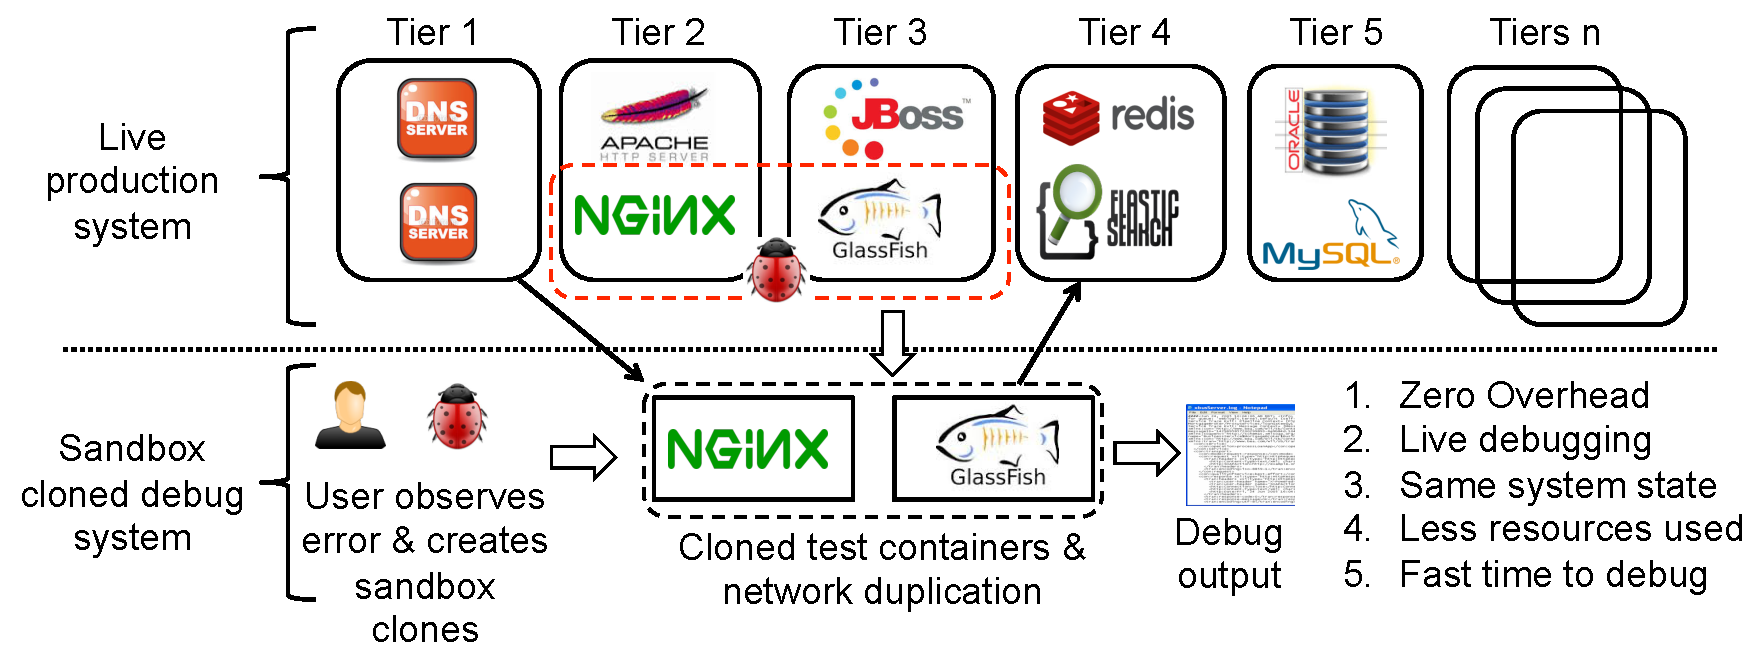
\includegraphics[width=0.99\textwidth]{parikshan/figs/workflow3.pdf}
		\caption{Workflow of \parikshan in a live multi-tier production system with several interacting services. When the administrator of the system observes errors in two of it's tiers, he can create a sandboxed clone of these tiers and observe/debug them in a sandbox environment without impacting the production system.}
		\label{fig:motivation}
	\end{center}
\end{figure*}